\documentclass[tikz, border=30pt]{standalone}
\usetikzlibrary{shapes.geometric, arrows.meta, positioning, fit, backgrounds, calc}

\begin{document}
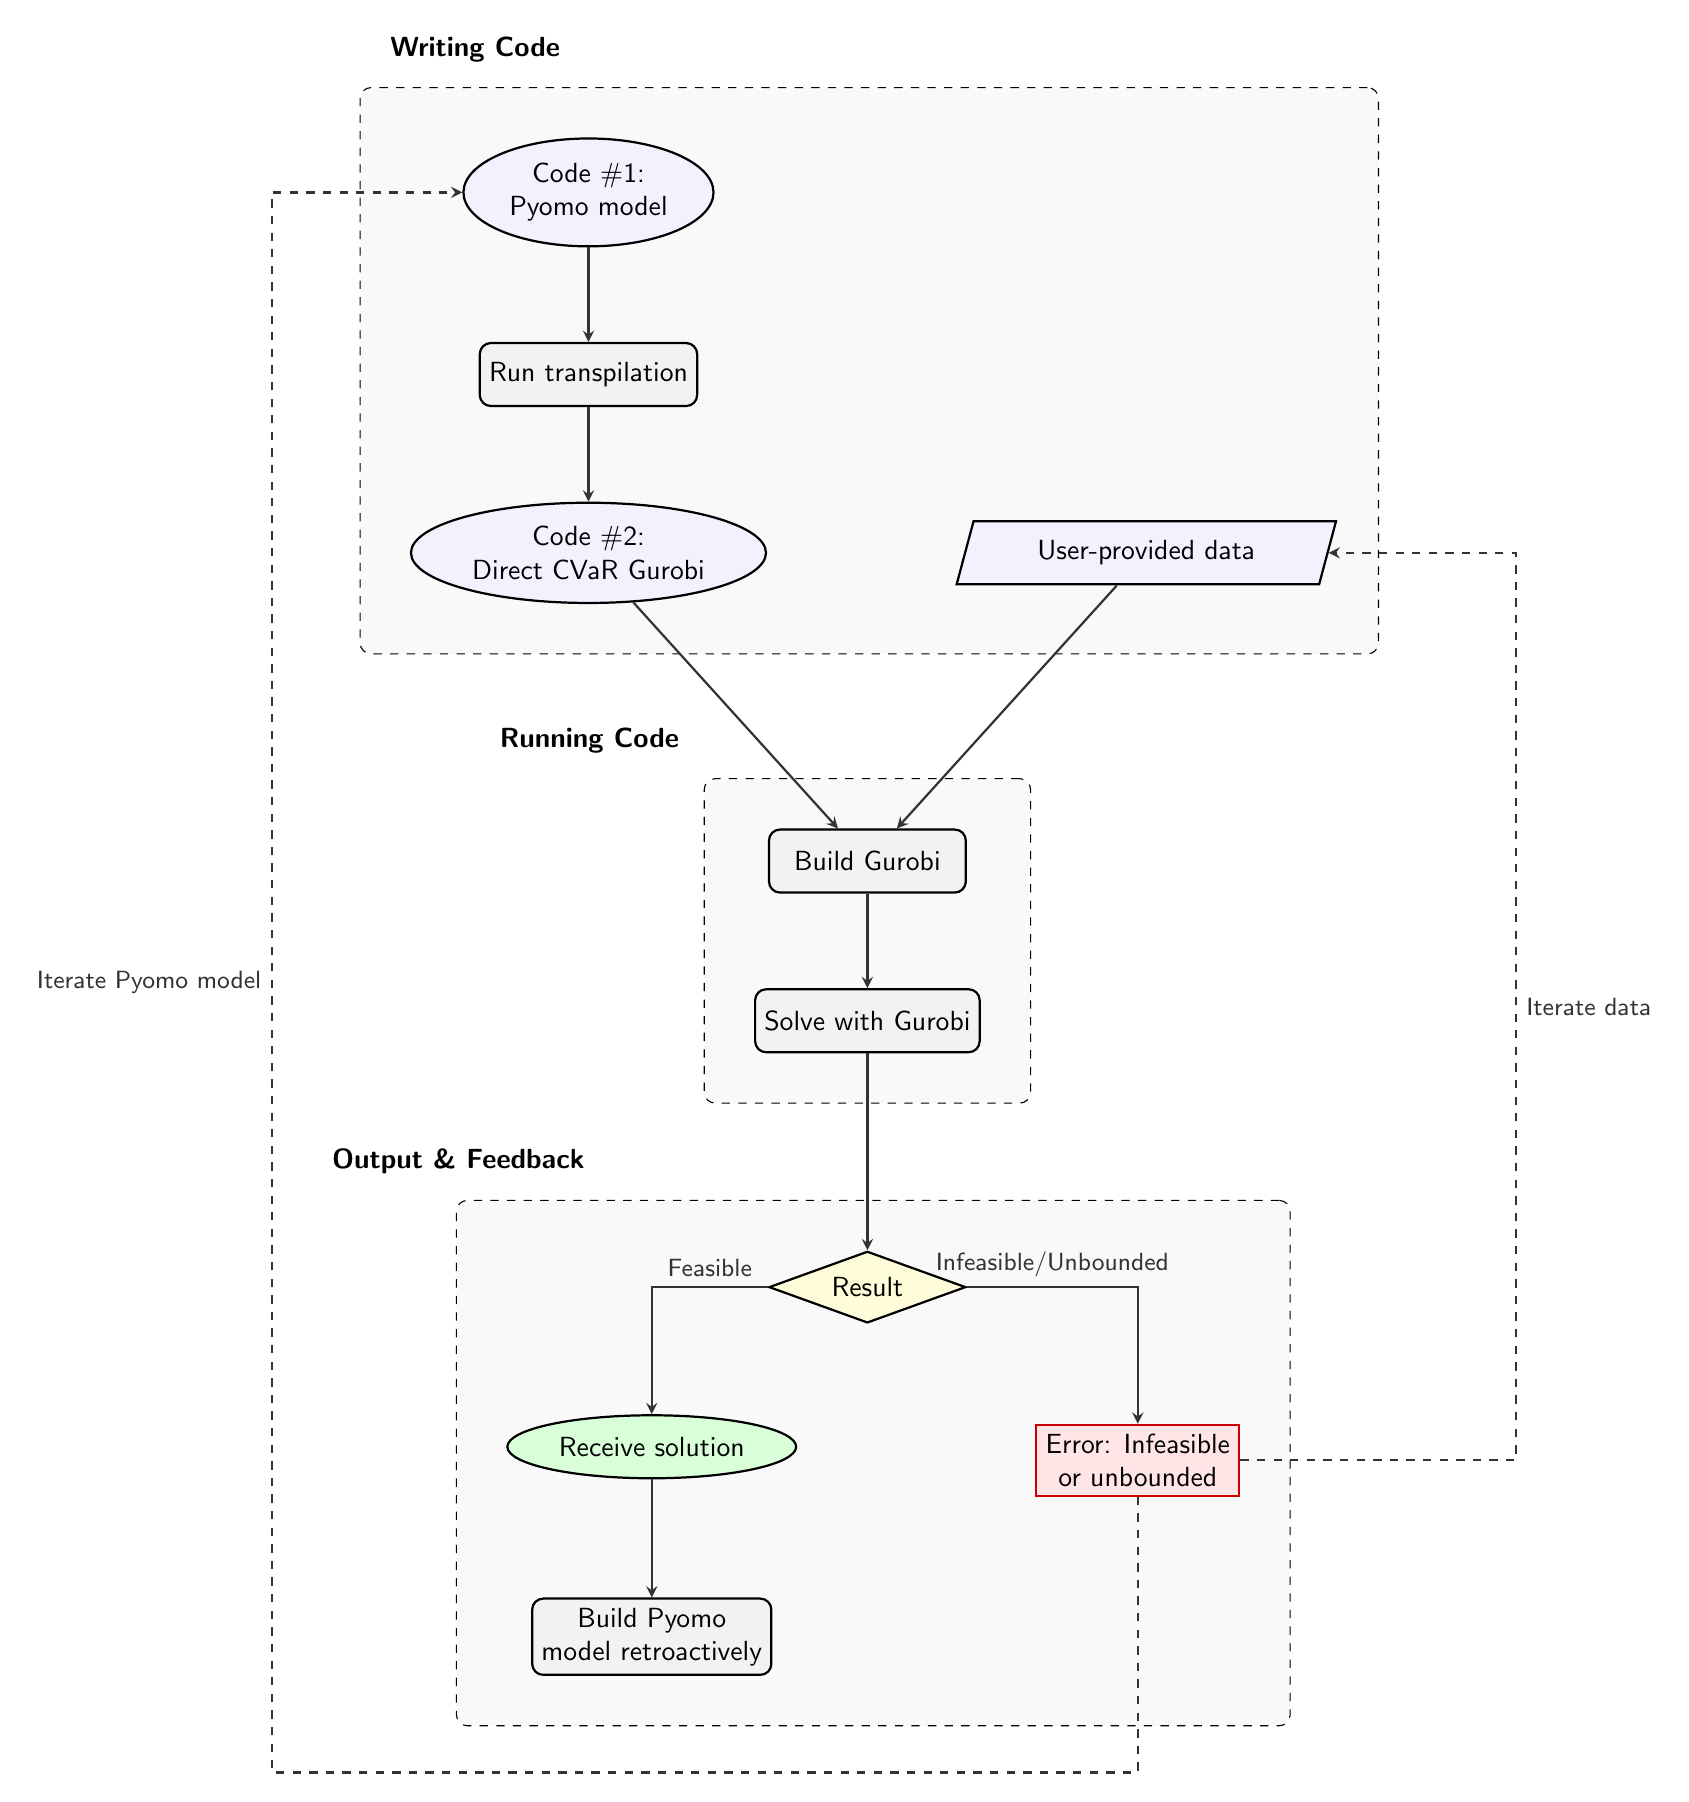
\begin{tikzpicture}[
    % --- STYLES ---
    base/.style={draw, thick, align=center, minimum height=0.8cm, minimum width=2.5cm, font=\sffamily},
    data/.style={base, trapezium, trapezium left angle=75, trapezium right angle=105, fill=blue!5},
    source/.style={base, ellipse, fill=blue!5},
    process/.style={base, rectangle, rounded corners, fill=gray!10},
    bottleneck/.style={process, fill=orange!15, draw=orange!90!black, thick},
    decision/.style={base, diamond, fill=yellow!15, aspect=2, inner sep=2pt},
    success/.style={base, ellipse, fill=green!15},
    error/.style={base, rectangle, fill=red!10, draw=red!80!black},
    container/.style={draw, dashed, rounded corners, inner sep=18pt, fill=gray!5},
    arrow/.style={->, >=stealth, thick, color=black!80},
    dashed arrow/.style={->, >=stealth, thick, dashed, color=black!80}
]

    % --- NODES ---
    
    % Phase 1: Writing Code (Loosened vertical spacing to 1.2cm)
    \node[source] (code1) {Code \#1:\\Pyomo model};
    \node[process, below=1.2cm of code1] (transpile) {Run transpilation};
    \node[source, below=1.2cm of transpile] (code2) {Code \#2:\\Direct CVaR Gurobi};
    
    % Pushed data wider to 2.5cm for breathing room
    \node[data, right=2.5cm of code2] (data) {User-provided data};

    % Phase 2: Running Code (Dropped 2.5cm below Phase 1)
    \node[process, below=3.5cm of $(code2)!0.5!(data)$] (build) {Build Gurobi};
    \node[process, below=1.2cm of build] (solve) {Solve with Gurobi};

    % Phase 3: Output & Feedback (Dropped 2.5cm below Phase 2)
    \node[decision, below=2.5cm of solve] (feedback) {Result};
    \node[success, below left=1.5cm and 0.8cm of feedback] (sol) {Receive solution};
    \node[error, below right=1.5cm and 1.5cm of feedback] (nosol) {Error: Infeasible\\ or unbounded};
    
    \node[process, below=1.5cm of sol] (optpyomo) {Build Pyomo\\model retroactively};

    % --- SUBGRAPHS ---
    \begin{scope}[on background layer]
        \node[container, fit=(code1)(transpile)(code2)(data), label={[font=\sffamily\bfseries, xshift=-2mm,yshift=2mm]above left:Writing Code}] (phase1) {};
        \node[container, fit=(build)(solve), label={[font=\sffamily\bfseries, xshift=-2mm, yshift=2mm]above left:Running Code}] (phase2) {};
        \node[container, fit=(feedback)(sol)(nosol)(optpyomo), label={[font=\sffamily\bfseries, xshift=-2mm, yshift=2mm]above left:Output \& Feedback}] (phase3) {};
    \end{scope}

    % --- FORWARD FLOW ---
    \draw[arrow] (code1) -- (transpile);
    \draw[arrow] (transpile) -- (code2);
    
    % V-Funnel into Build
    \draw[arrow] (code2) -- (build);
    \draw[arrow] (data) -- (build);
    
    \draw[arrow] (build) -- (solve);
    \draw[arrow] (solve) -- (feedback);
    
    \draw[arrow] (feedback) -| node[above, near start, font=\sffamily\small] {Feasible} (sol);
    \draw[arrow] (feedback) -| node[above, near start, font=\sffamily\small] {Infeasible/Unbounded} (nosol);

    \draw[arrow] (sol) -- (optpyomo);

    % --- FEEDBACK LOOPS ---
    
    % Right Loop: Iterating Data (Pushed wider to ++(3.5,0) so it stays well clear of the boxes)
    \draw[dashed arrow] (nosol.east) -- ++(3.5,0) |- node[pos=0.25, right, font=\sffamily\small] {Iterate data} (data.east);
    
    % Left Loop: Iterating Pyomo Model 
    % Dropped lower to ++(0,-2.5) to cleanly sweep under the Optional Pyomo block, and swept wider left to ++(-11,0)
    \draw[dashed arrow] (nosol.south) -- ++(0,-3.5) -| ++(-11,0) |- node[pos=0.25, left, font=\sffamily\small] {Iterate Pyomo model} (code1.west);

\end{tikzpicture}
\end{document}